
\begin{table}[t]
\caption{Quantitative comparisons on Tiktok dataset.}
\vspace{5pt}
\label{tab: tiktok exp}
\scriptsize
\centering
\setlength{\tabcolsep}{1pt}
\begin{tabular}{lccccccccc}
\toprule
\multirow{3}{*}{\textbf{Method}} & \multicolumn{6}{c}{\textbf{VBench}$\uparrow$} & \multirow{3}{*}{\textbf{FID-FVD}$\downarrow$} & \multirow{3}{*}{\textbf{FVD}$\downarrow$} & \multirow{3}{*}{\textbf{CD-FVD}$\downarrow$} \\ \cmidrule{2-7}
                        & \textbf{Temporal}   & \textbf{Subject}      & \textbf{Background} & \textbf{Motion} & \textbf{Dynamic} & \textbf{Imaging} \\
                        & \textbf{Flickering}     & \textbf{Consistency}  & \textbf{Consistency} & \textbf{Smoothness} & \textbf{Degree} & \textbf{Quality} \\
\midrule
\multicolumn{9}{l}{\color{gray}{\emph{Stable Diffusion1.5}}}\\
MagicPose~\citep{chang2023magicpose} & 96.65 & 95.12 & 94.55 & 98.29 & 22.70 & 63.87 & 15.53 & 1015.04 & 693.24\\
Moore~\citep{moore-animateanyone}	& 96.86 & 95.18 & 95.37 & 98.01 & 25.51 & 69.14 & 11.58 & 924.40 & 687.88\\
MusePose~\citep{musepose} & 97.02 & 95.27 & 95.16 & 98.45 & 27.31 & 71.56 & 11.48 & 866.36 & 626.59\\
\rowcolor{aliceblue!60}
MusePose+Ours	& \textbf{97.63} & \textbf{95.70} & \textbf{95.64} & \textbf{98.51} & \textbf{31.34} & \textbf{71.89} & \textbf{11.26} & \textbf{764.00} &\textbf{622.64}\\
\midrule
\multicolumn{9}{l}{\color{gray}{\emph{Stable Video Diffusion}}}\\
ControlNeXt~\citep{peng2024controlnext}	& 97.55 & 94.58 & 95.60 & 98.75 & 27.58 & 70.40 & 10.49 & 496.87&624.51 \\
MimicMotion~\citep{zhang2024mimicmotion}	& 97.56 & 94.95 & 95.36 & 98.67 & 28.42 & 68.42 & 10.50 & 598.41&621.90 \\
\rowcolor{aliceblue!60}
MimicMotion+Ours & \textbf{97.73} & \textbf{95.72} & \textbf{95.90} & \textbf{98.89} & \textbf{29.51} & \textbf{71.33} & \textbf{10.24} & \textbf{466.93} &\textbf{603.27}\\
\bottomrule
\end{tabular}
\vspace{-5pt}
\end{table}



\begin{table}[t]
\caption{Quantitative comparisons on unseen dataset.}
\vspace{5pt}
\scriptsize
\centering
\setlength{\tabcolsep}{5pt}
\begin{tabular}{lccccccc}
\toprule		
\multirow{2}{*}{\textbf{Method}}
                        & \textbf{Temporal}    & \textbf{Subject}      & \textbf{Background} & \textbf{Motion} & \textbf{Dynamic} & \textbf{Imaging} & \textbf{Aesthetic} \\
                         & \textbf{Flickering}    & \textbf{Consistency}  & \textbf{Consistency} & \textbf{Smoothness} & \textbf{Degree} & \textbf{Quality} & \textbf{Quality} \\
\midrule
\multicolumn{8}{l}{\color{gray}{\emph{Stable Diffusion1.5}}} \\
MagicPose~\citep{chang2023magicpose}  & 92.65& 93.71 & 98.51 & 25.67 & 63.78 & 93.65 & 46.16\\
Moore~\citep{moore-animateanyone}  & 92.83 & 92.42 & 98.12 & 27.43 & 65.32 & 94.61& 47.23\\
MusePose~\citep{musepose}  & 93.12 & 93.97 & 98.58 & 28.72 & 65.26 & 96.41 & 49.34\\
\rowcolor{aliceblue!60}
MusePose+Ours	 &  \textbf{93.43} & \textbf{94.22} & \textbf{98.76} & \textbf{29.61} & \textbf{65.48} & \textbf{96.63} & \textbf{49.39} \\
\midrule
\multicolumn{8}{l}{\color{gray}{\emph{Stable Video Diffusion}}} \\
ControlNeXt~\citep{peng2024controlnext}	 & 93.25 & 94.27 & 98.70 & 28.42 & 64.36 & 97.42 & 49.10 \\
MimicMotion~\citep{zhang2024mimicmotion}	 & 93.32 & 94.12 & 98.50 & 29.81 & 64.51 & 97.45 & 49.03 \\
\rowcolor{aliceblue!60}
MimicMotion+Ours  & \textbf{93.59} & \textbf{94.35}& \textbf{98.75}& \textbf{30.02} & \textbf{65.56}& \textbf{97.80}  & \textbf{49.93}\\
\bottomrule
\end{tabular}
\label{tab: ood exp}
% \vspace{-5pt}
\end{table}

\section{Experiments}
\subsection{Implementations}
\textbf{Baseline Models.}
To demonstrate the effectiveness of DisPose, we integrate the proposed modules into two open-source human image animation models: MusePose~\citep{musepose} and MimicMotion~\citep{zhang2024mimicmotion}.
MusePose~\citep{musepose} is a reimplementation of AnimateAnyone~\citep{hu2023animate} by optimizing Moore-AnimateAnyone~\citep{moore-animateanyone}, which implements most of the details of AnimateAnyone~\citep{hu2023animate} and achieves comparable performance. MimicMotion~\citep{zhang2024mimicmotion} is the state-of-the-art human animation model based on Stable Video Diffusion~\citep{blattmann2023svd}.

\textbf{Implementation Details.} Following~\citep{hu2023animate,zhang2024mimicmotion}, We employed DWPose~\citep{yang2023dwpose} to extract the pose sequence of characters in the video and render it as pose skeleton images following OpenPose~\citep{cao2017openpose}. We collected 3k human videos from the internet to train our model. For MusePose~\citep{musepose}, we used \texttt{stable-diffusion-v1-5}\footnote{\hyperlink{https://huggingface.co/stable-diffusion-v1-5/stable-diffusion-v1-5}{https://huggingface.co/stable-diffusion-v1-5/stable-diffusion-v1-5}.} to initialize our hybrid ControlNet. We sampled 16 frames from each video and center cropped to a resolution of 512×512. Training was conducted for 20,000 steps with a batch size of 32. The learning rate was set to 1e-5. For MimicMotion~\citep{zhang2024mimicmotion}, we initialized our hybrid ControlNet using \texttt{stable-video-diffusion-img2vid-xt-1-1}\footnote{\hyperlink{https://huggingface.co/stabilityai/stabilityai/stable-video-diffusion-img2vid-xt-1-1}{https://huggingface.co/stabilityai/stabilityai/stable-video-diffusion-img2vid-xt-1-1}.}. We sampled 16 frames from each video and center crop to a resolution of 768×1024. Training was conducted for 10,000 steps with a batch size of 8. The learning rate was set to 2e-5.

\textbf{Evaluation metrics.} The video quality is evaluated by calculating {the Frechet Inception Distance with Fréchet Video Distance (FID-FVD)~\citep{balaji2019fid-fvd}, Fréchet Video Distance (FVD)~\citep{unterthiner2018fvd} and Content-Debiased Fréchet Video Distance (CD-FVD)~\citep{ge2024content}}
between the generated video and the grounded video. Considering that these metrics are inconsistent with human judgment~\citep{huang2024vbench}, we introduce metrics in VBench~\citep{huang2024vbench} to comprehensively assess the consistency of the generated video with human perception, including temporal flickering, aesthetic quality, subject consistency, background consistency, motion smoothness, dynamic degree, and imaging quality.

\begin{figure}[t]
    \centering
    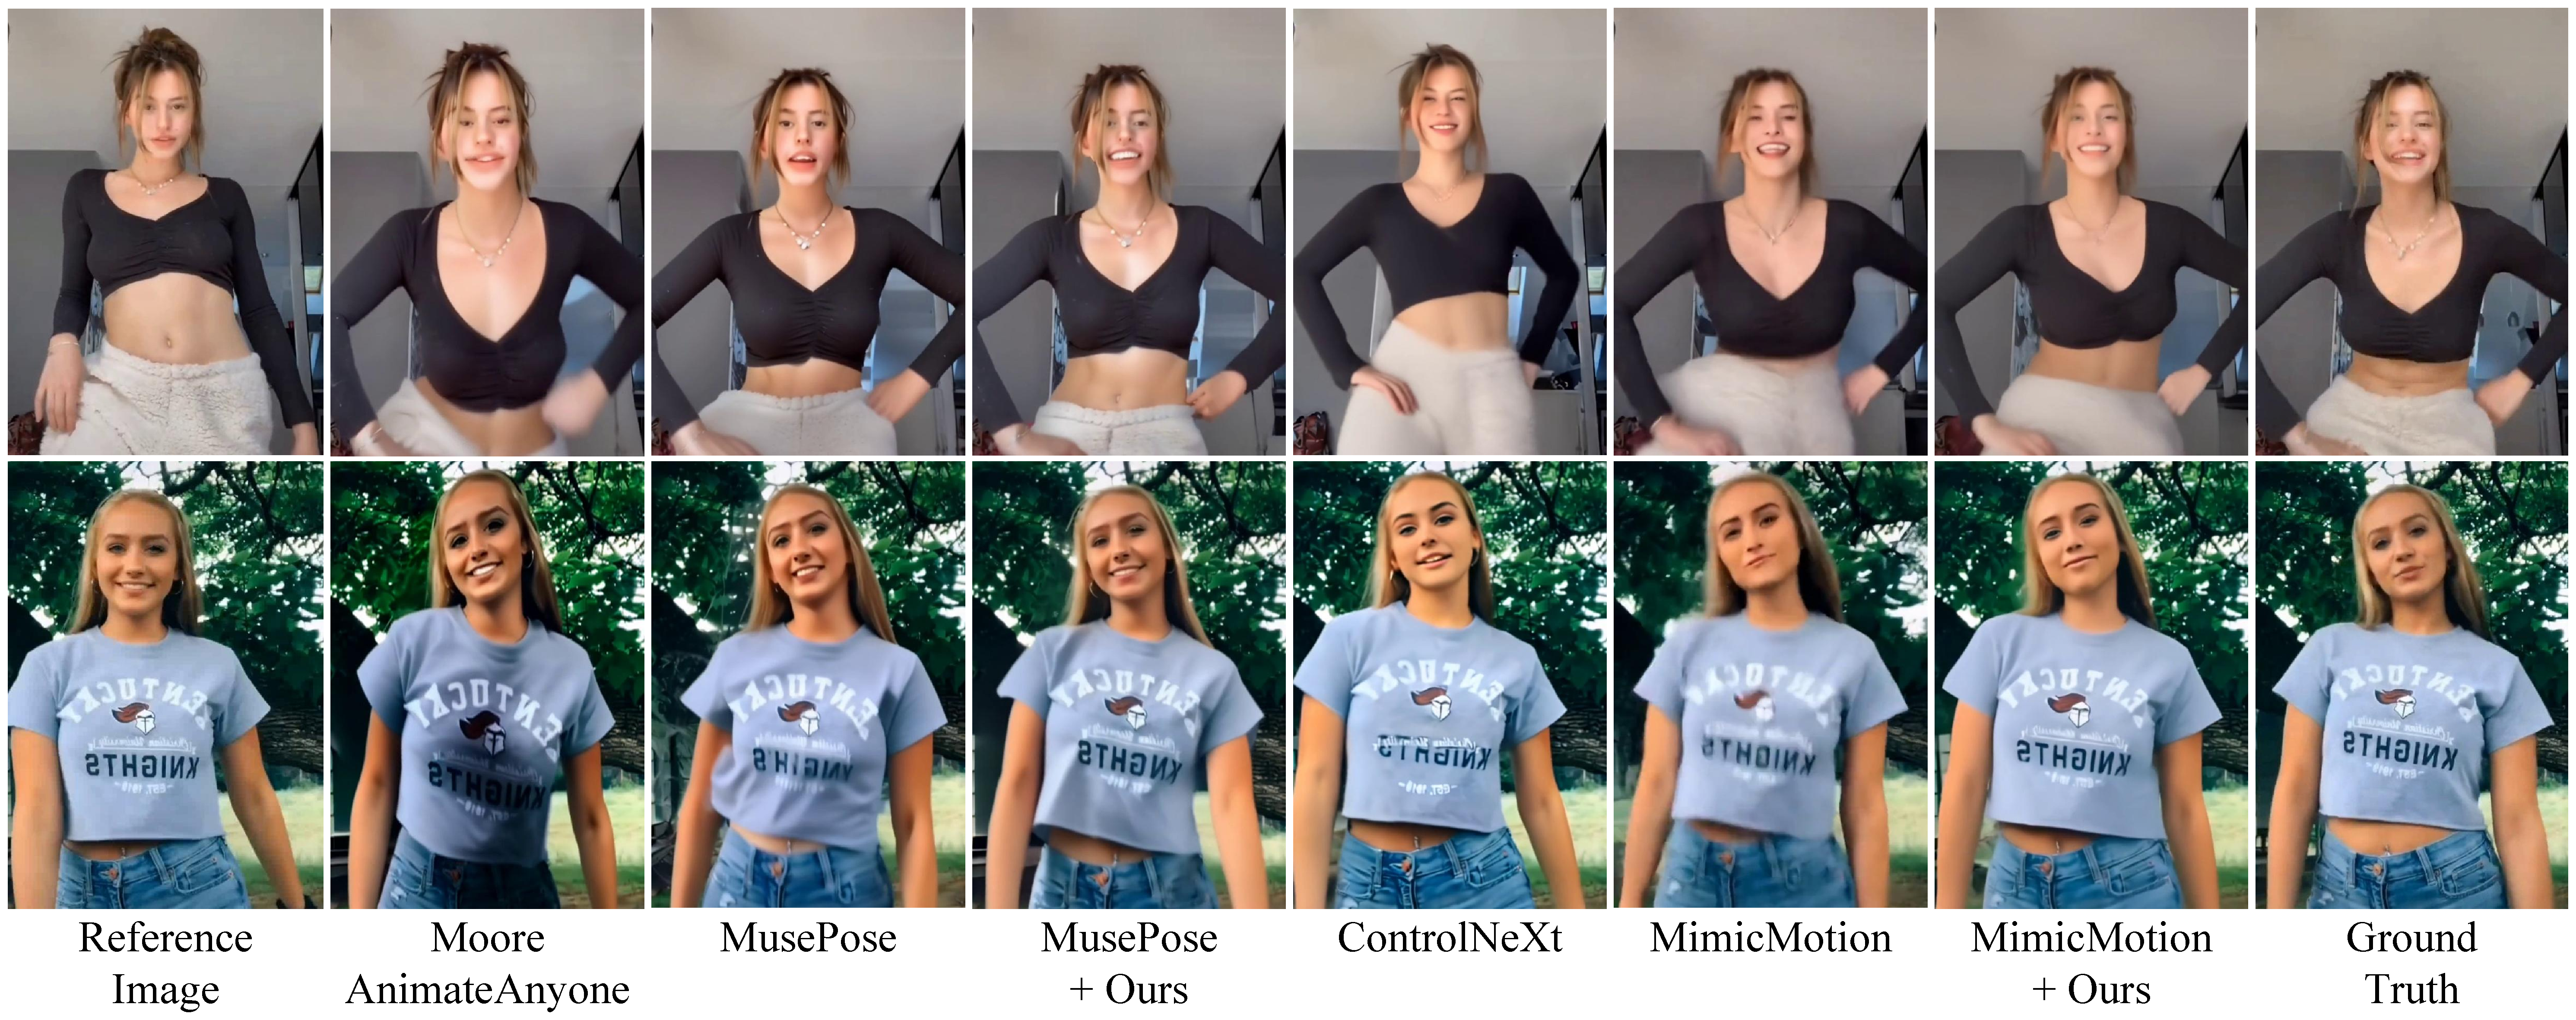
\includegraphics[width=1.0\columnwidth]{./image/exp2.pdf}
    \vspace{-20pt}
    \caption{Qualitative comparisons between our method and the state-of-the-art models on the TikTok dataset.}
    \label{fig: vis tiktok}
    % \vspace{-5pt}
\end{figure}

\begin{figure}[t]
    \centering
    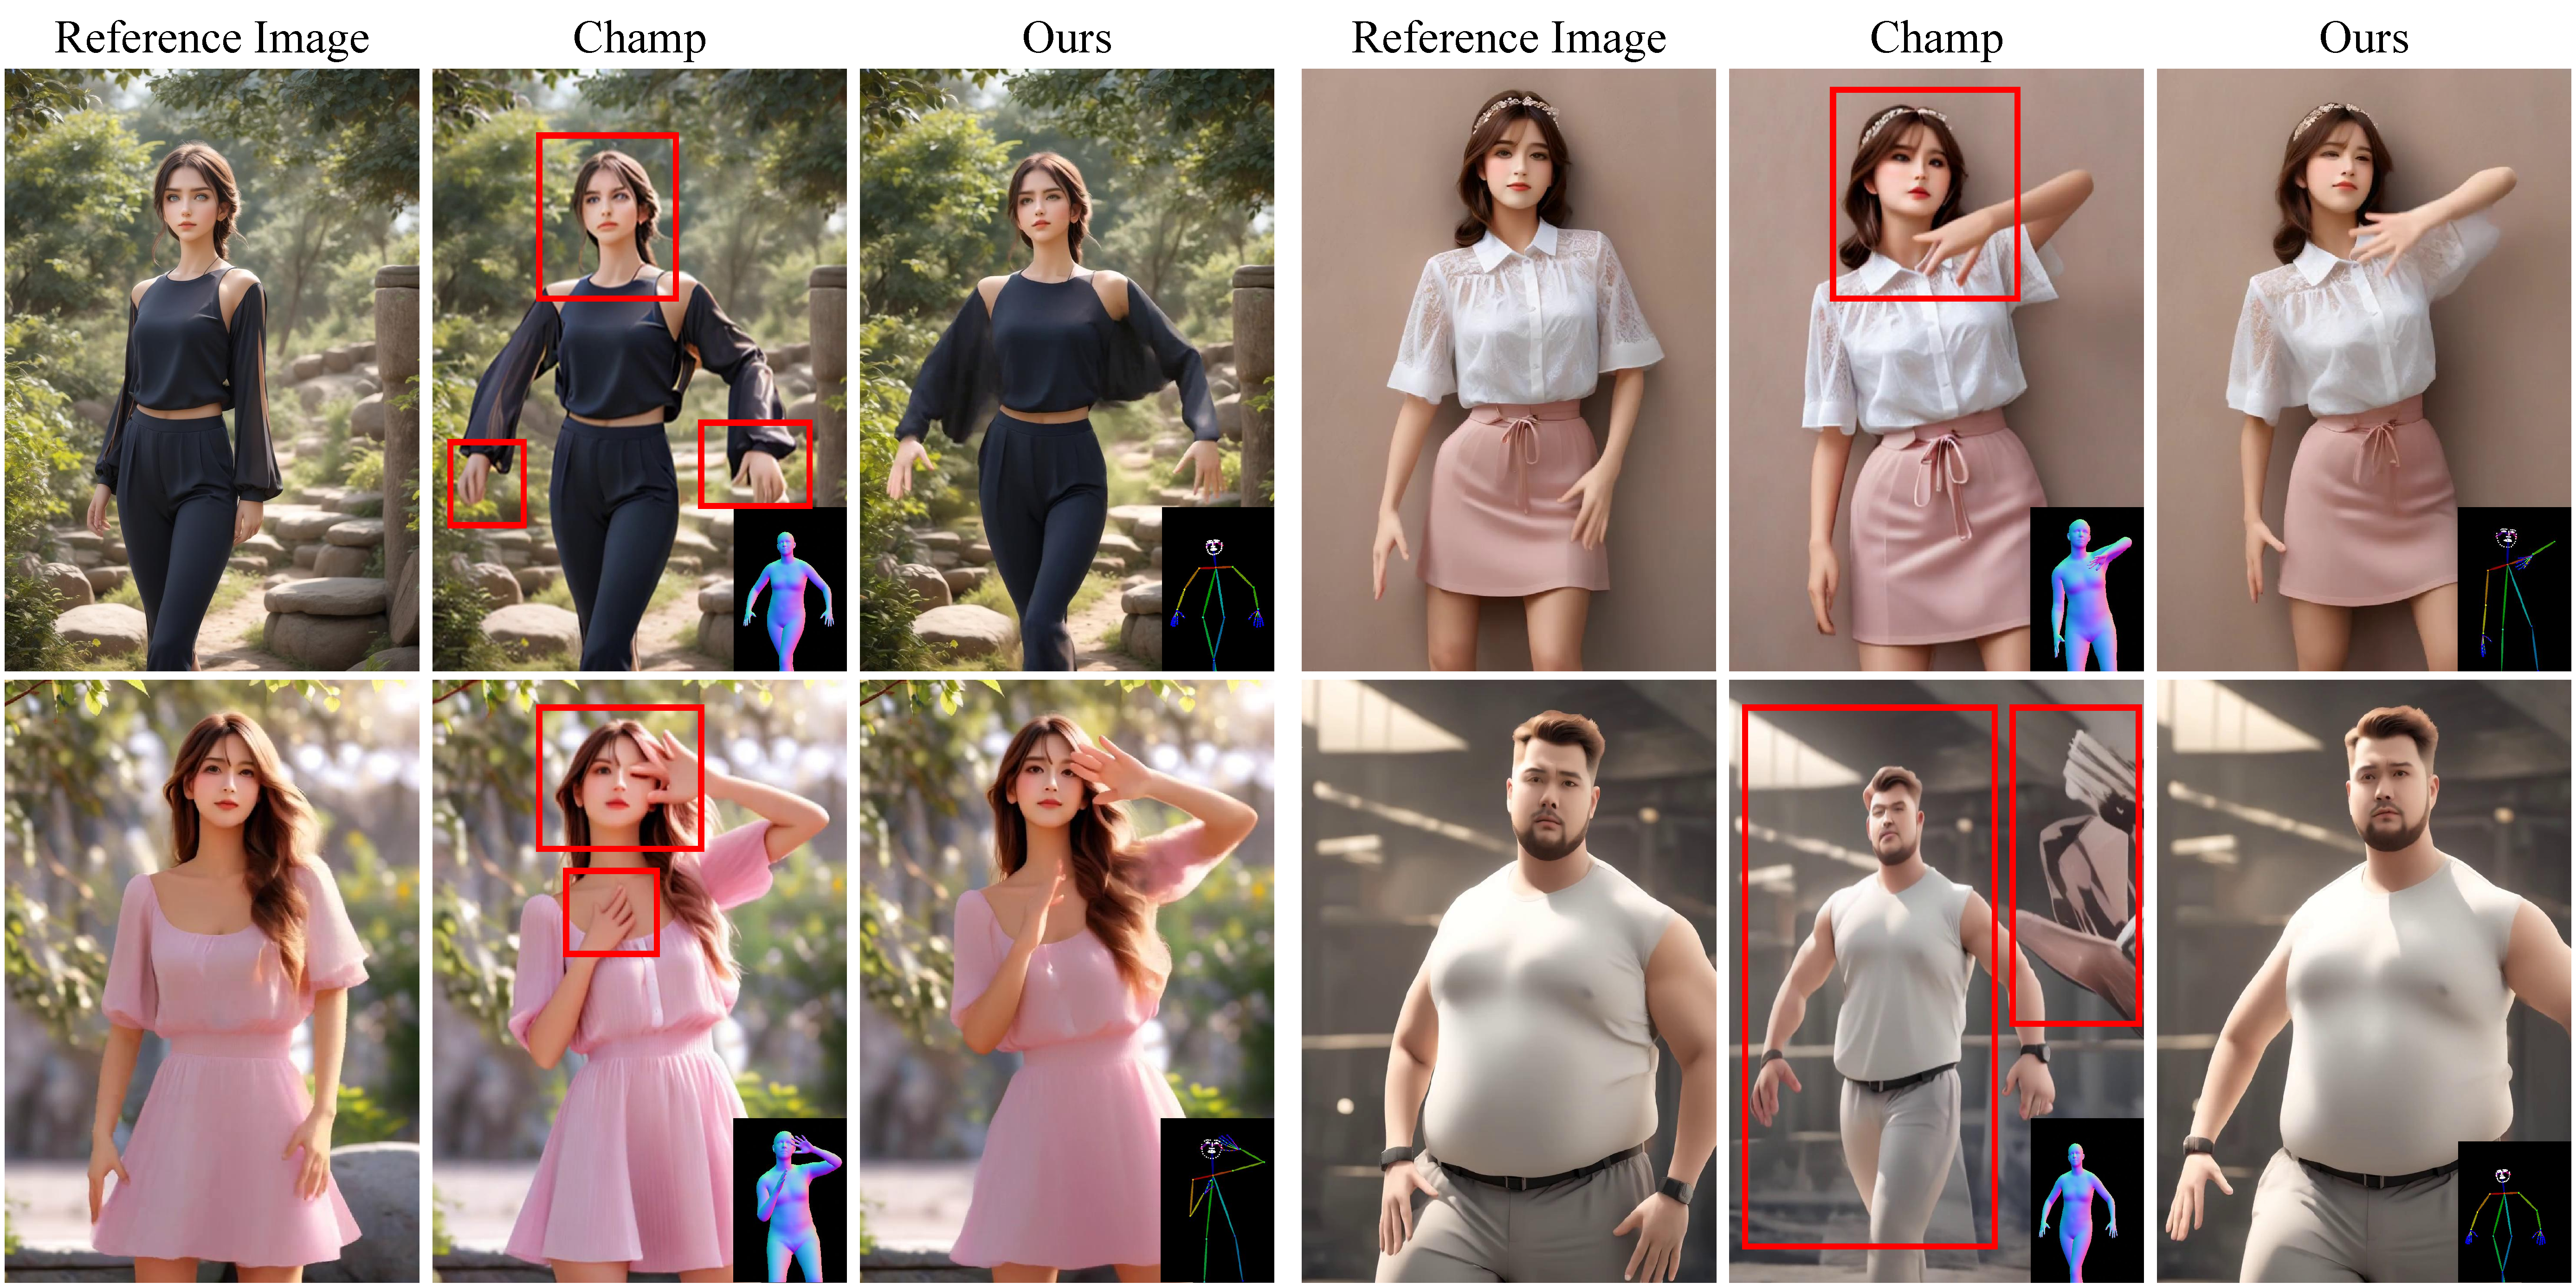
\includegraphics[width=1.0\columnwidth]{./image/exp.pdf}
    \vspace{-20pt}
    \caption{Qualitative comparison of our approach with the dense control-based method.}
    \label{fig: com_champ}
\end{figure}

% \subsection{Comparisons with State-of-the-Art Methods}
\subsection{Quantitative Comparison}
\textbf{Evaluation on TikTok dataset.}
We compare our method to the state-of-the-art human image animation methods, including MagicPose~\citep{chang2023magicpose}, Moore-AnymateAnyone~\citep{moore-animateanyone}, MusePose~\citep{musepose}, ControlNeXt~\citep{peng2024controlnext} and MimicMotion~\citep{zhang2024mimicmotion}. Following previous works~\citep{zhang2024mimicmotion,wang2024disco}, we use sequences 335 to 340 from the TikTok~\citep{jafarian2021tiktok} dataset for testing.
Table~\ref{tab: tiktok exp} presents a quantitative analysis of the various methods evaluated on the TikTok dataset. The proposed methods achieve significant improvements across different baseline models. Our method achieves higher scores on VBench~\citep{huang2024vbench} while reducing FID-FVD and FVD scores, which indicates that the proposed method generates high-quality videos that align with human perception.


\textbf{Evaluation on unseen dataset.}
Training videos collected from the Internet may exhibit domain proximity with the TikTok~\citep{jafarian2021tiktok} test set. We construct an unseen dataset to further compare the generalizability of various methods. We collect 30 high-quality human videos and generate reference images with diverse styles using InstanID~\citep{wang2024instantid}. Due to the unavailability of the ground truth corresponding to the generated reference images, we use VBench~\citep{huang2024vbench} as the quantitative metric as shown in Table~\ref{tab: ood exp}.


\subsection{Qualitative Results}
\textbf{Comparison with state-of-the-art methods.}
Figure~\ref{fig: vis tiktok} illustrates the qualitative results between the various models on the TikTok dataset. Thanks to the motion field guidance and keypoint correspondence, our method can produce reasonable results with significant pose variation.

\begin{table}[t]
\caption{Ablation study on different control guidance. ``w/o Motion'' denotes the model configuration that disregards motion filed guidance. ``w/o Point'' indicates the variant model that removes the keypoint correspondence.}
\vspace{5pt}
\scriptsize
\centering
\setlength{\tabcolsep}{4pt}
\begin{tabular}{lcccccccc}
\toprule		
\multirow{3}{*}{\textbf{Method}} & \multicolumn{6}{c}{\textbf{VBench}$\uparrow$} & \multirow{3}{*}{\textbf{FID-FVD}$\downarrow$} & \multirow{3}{*}{\textbf{FVD}$\downarrow$} \\ \cmidrule{2-7}
                        & \textbf{Temporal}   & \textbf{Subject}      & \textbf{Background} & \textbf{Motion} & \textbf{Dynamic} & \textbf{Imaging} \\
                        & \textbf{Flickering}     & \textbf{Consistency}  & \textbf{Consistency} & \textbf{Smoothness} & \textbf{Degree} & \textbf{Quality} \\
\midrule
w/o Motion & 97.66 & 95.04 & 95.31 & 98.75 & 29.42 & 69.53 & 10.31 & 478.91\\
w/o Point & 97.47 & 95.57 & 95.43 & 98.42 & 29.14 & 70.14 & 10.28 & 498.74\\
\rowcolor{aliceblue!60}
Full Model & \textbf{97.73} & \textbf{95.72} & \textbf{95.90} & \textbf{98.89} & \textbf{29.51} & \textbf{71.33} & \textbf{10.24} & \textbf{466.93} \\
\bottomrule
\end{tabular}
\label{tab: abs}
% \vspace{-5pt}
\end{table}

\begin{figure}[t]
    \centering
    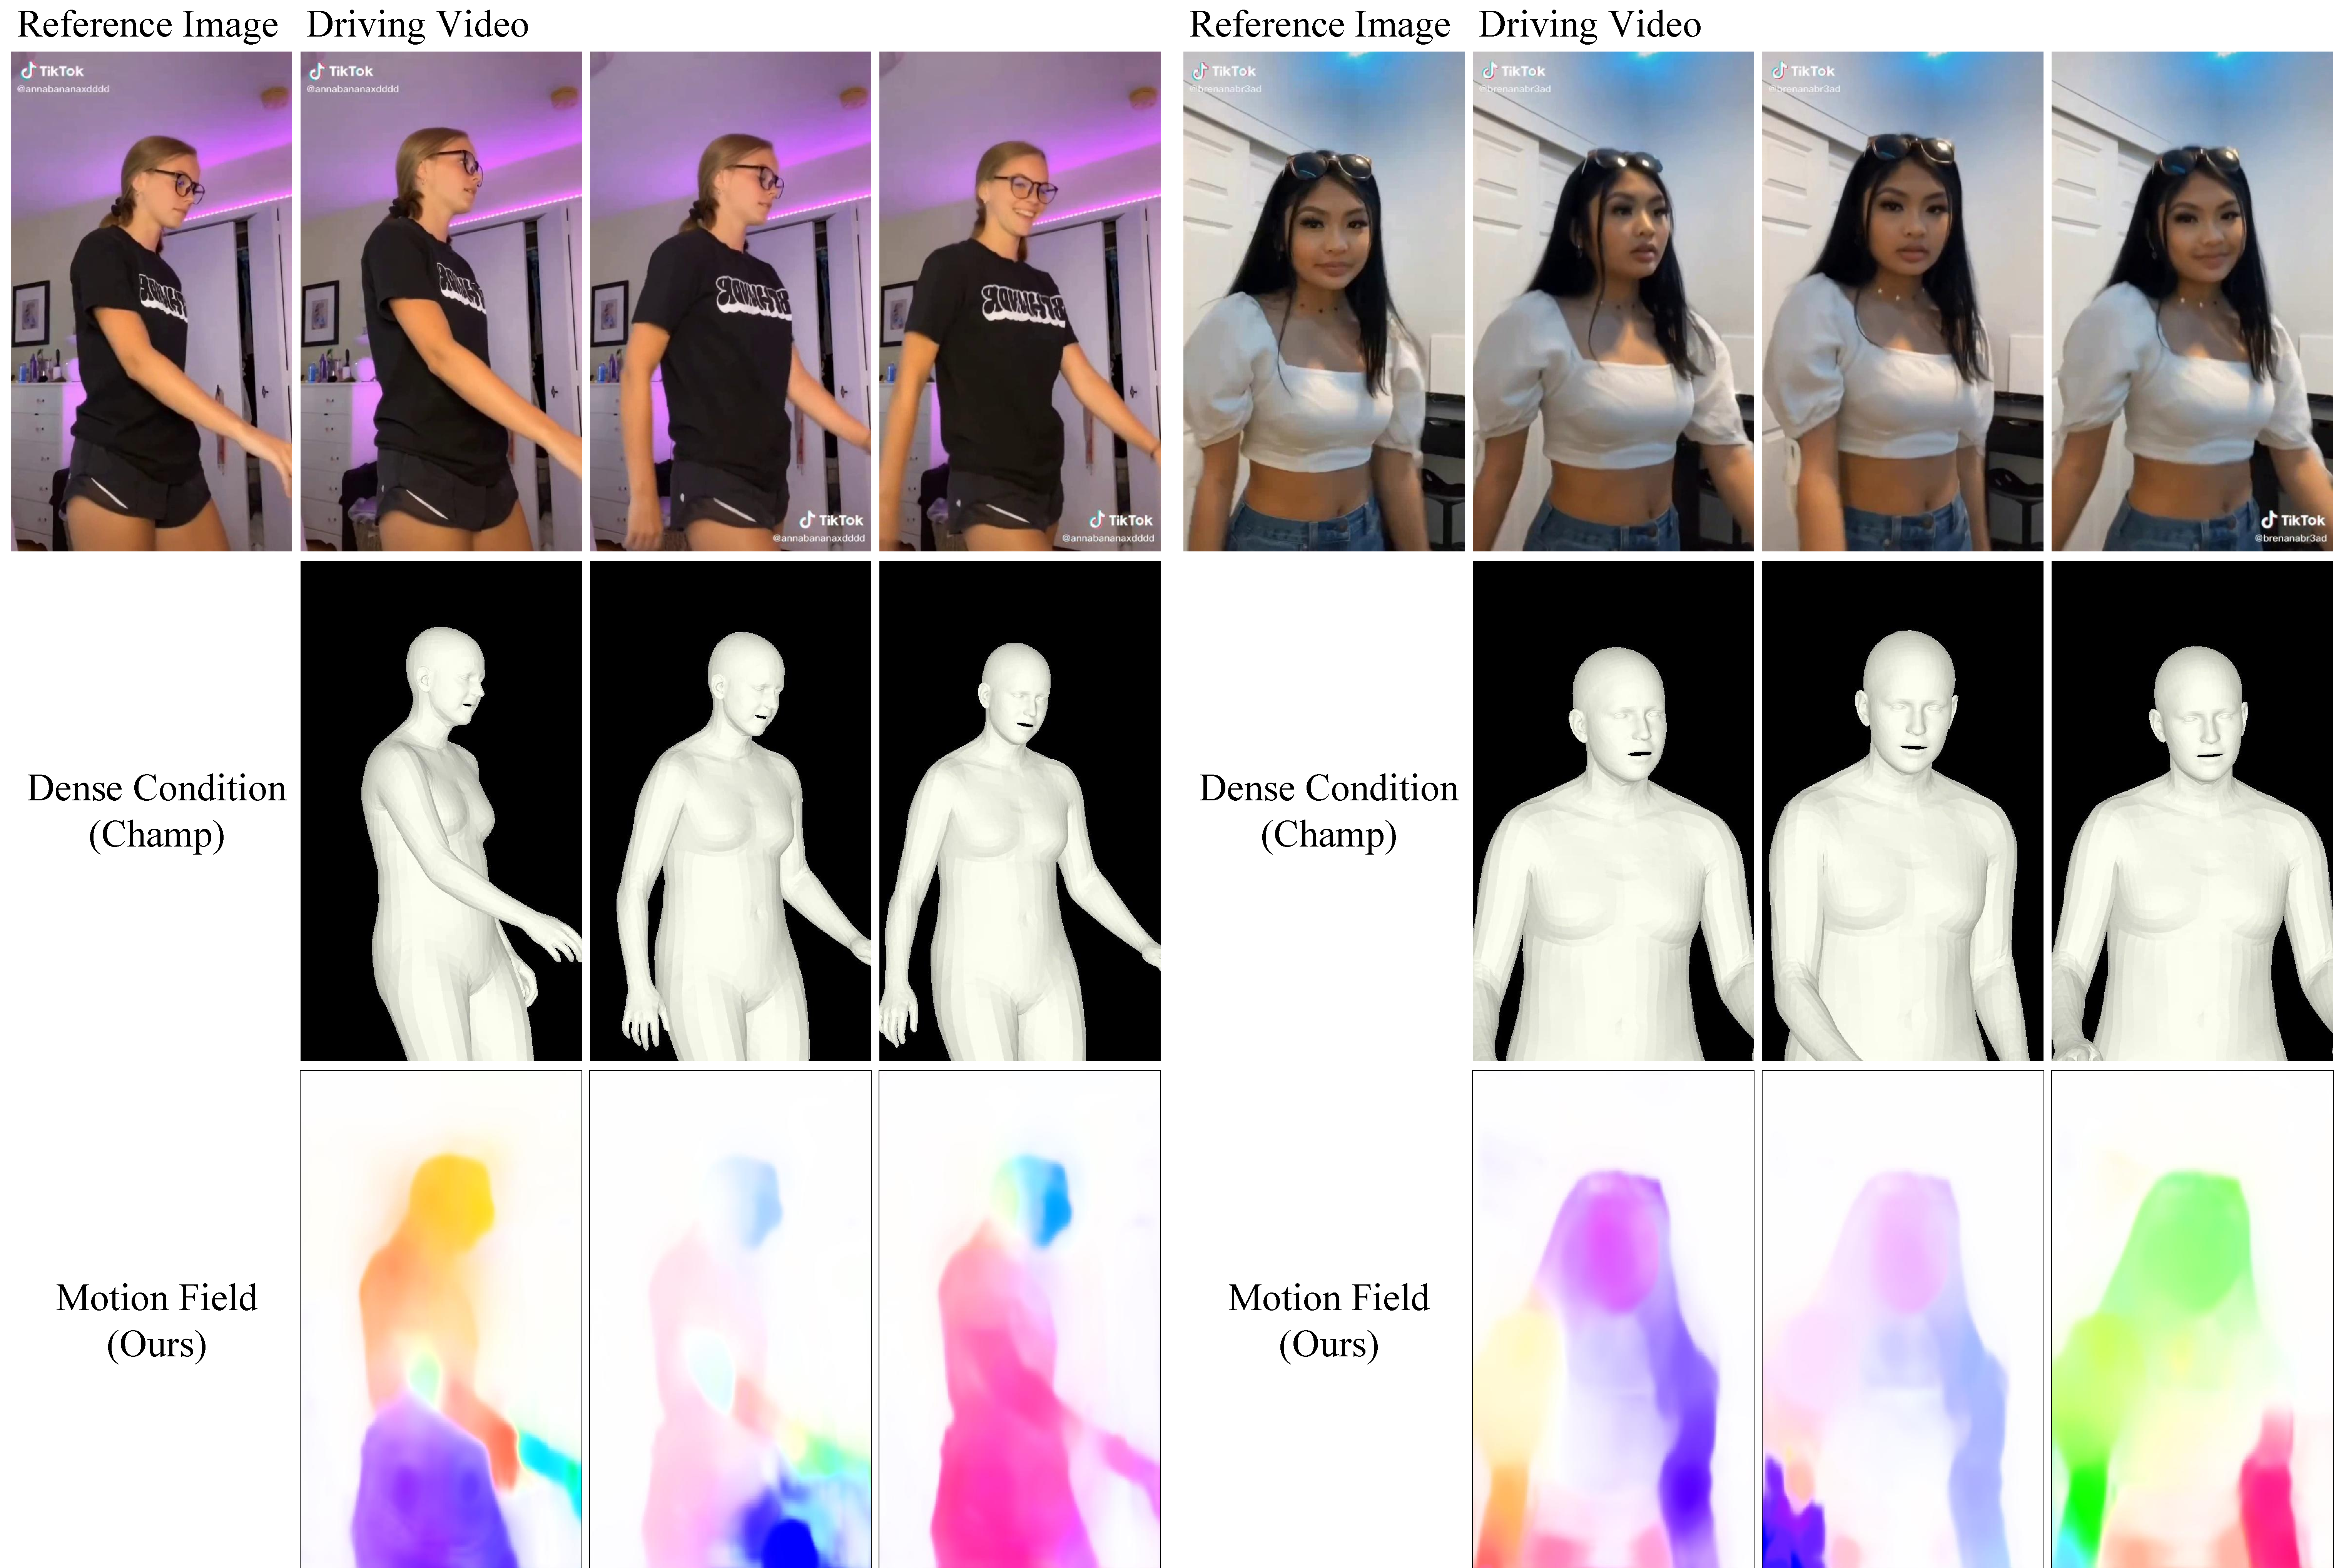
\includegraphics[width=1.0\columnwidth]{./image/exp4.pdf}
    \vspace{-20pt}
    \caption{Comparison of our reference-based dense motion field and existing dense conditions.}
    \label{fig: com_dense}
\end{figure}

\begin{figure}[t]
    \centering
    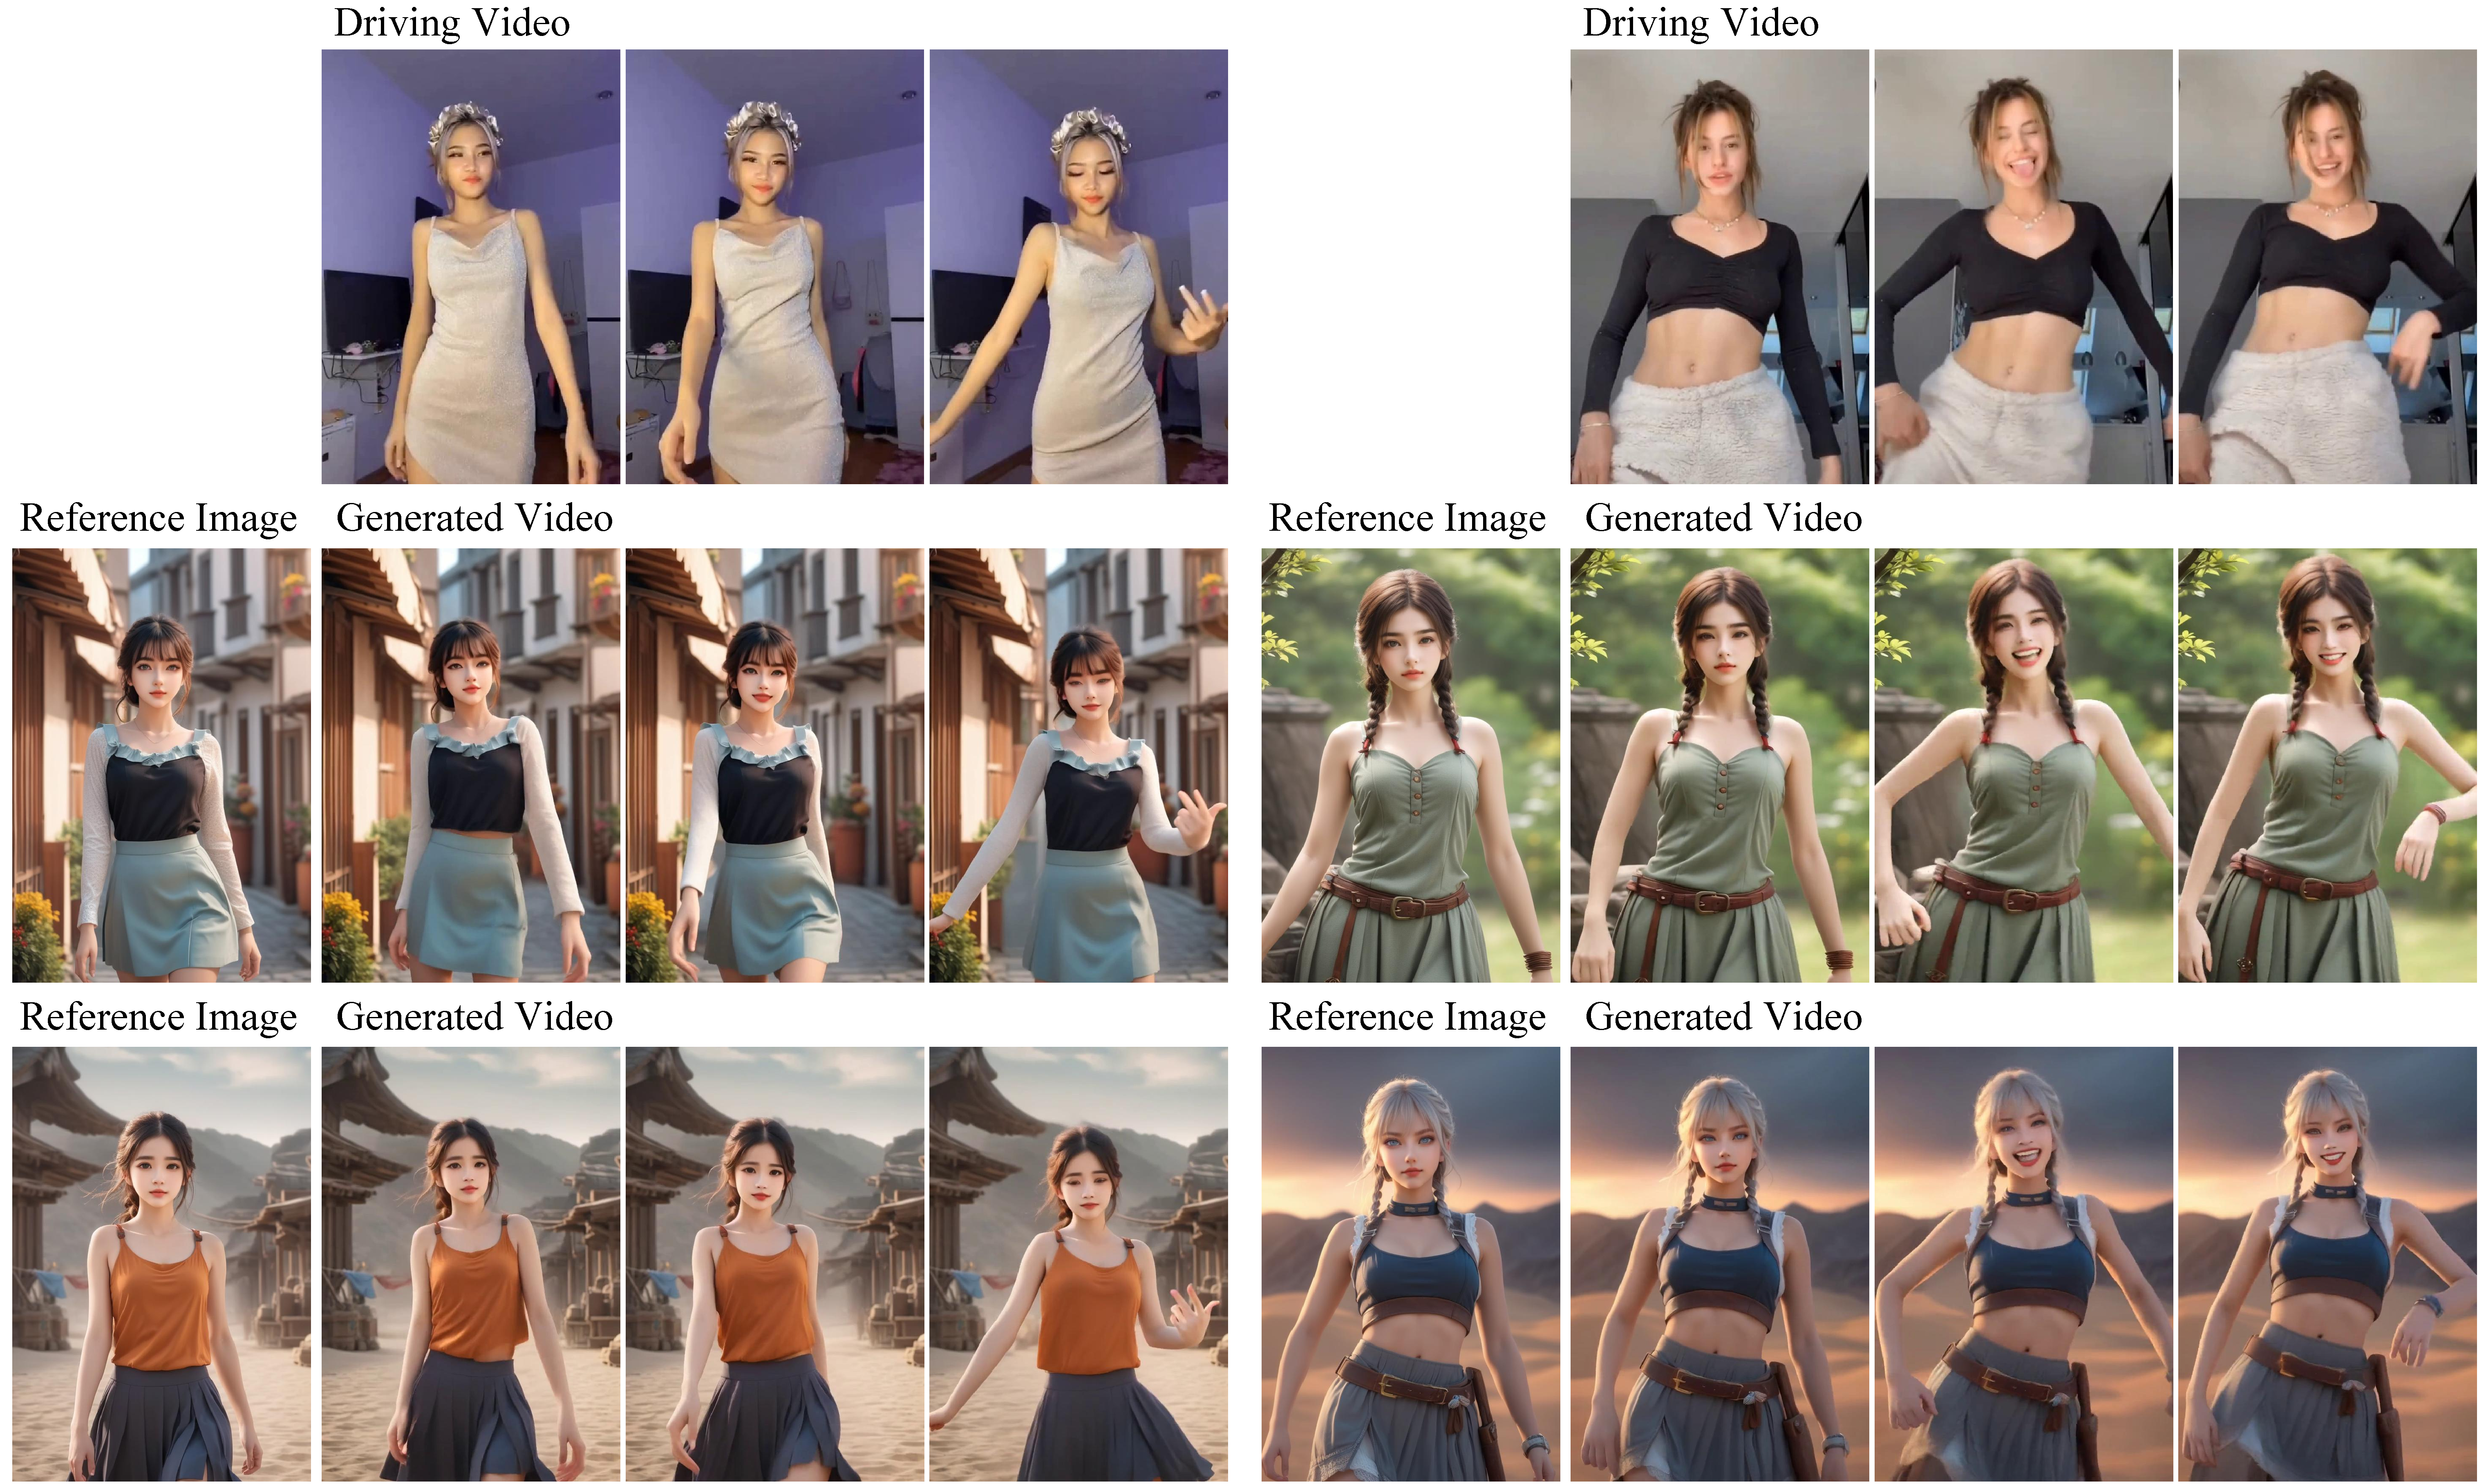
\includegraphics[width=1.0\columnwidth]{./image/exp3.pdf}
    \vspace{-20pt}
    \caption{The demonstration of cross ID animation from the proposed method.}
    \label{fig: cross_id}
\end{figure}
\vspace{-10pt}

\begin{figure}[t]
    \centering
    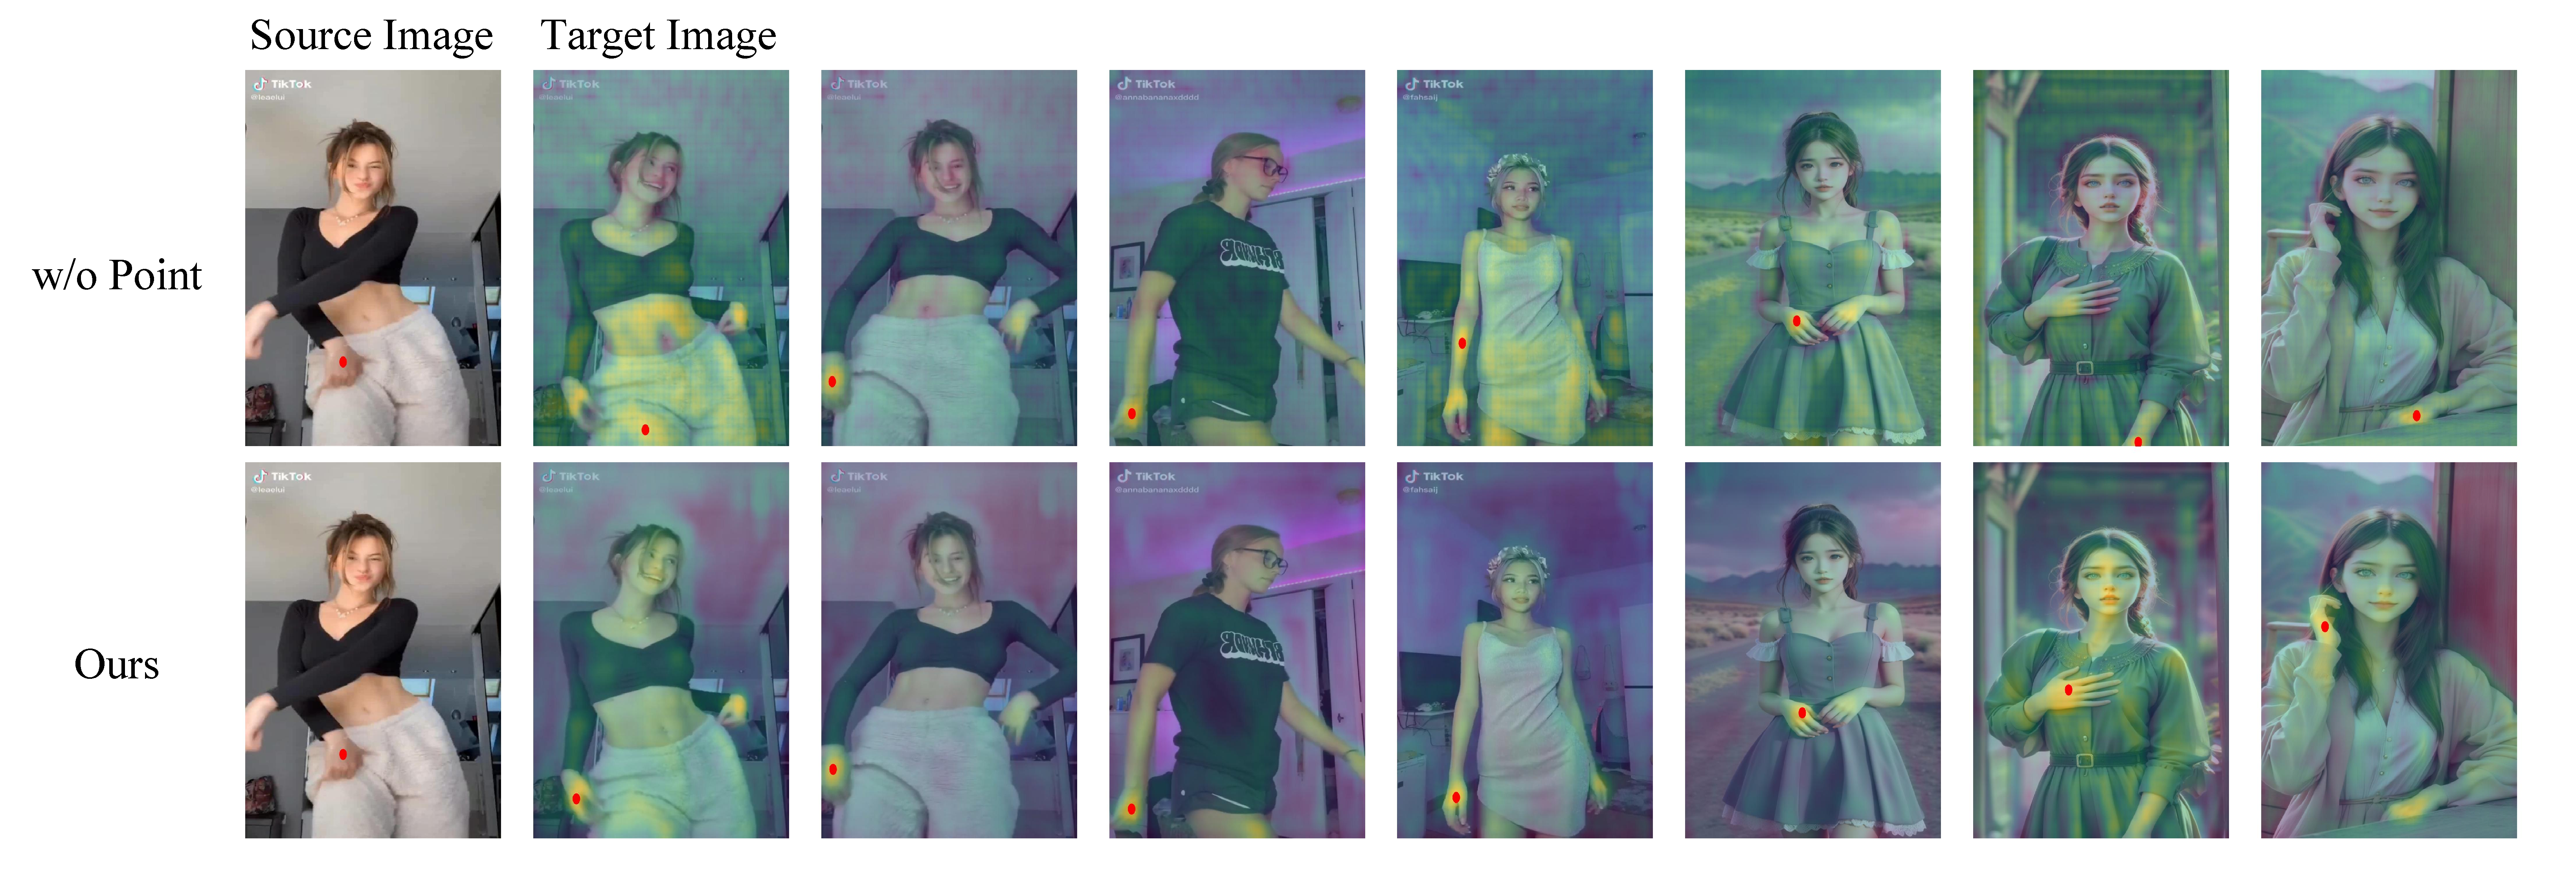
\includegraphics[width=1.0\columnwidth]{./image/cross_vis.pdf}
    \vspace{-20pt}
    \caption{Qualitative analysis of semantic correspondence. Given a red source point in an image (far left), we use its diffusion feature to retrieve the corresponding point in the image on the right.}
    \label{fig: point_abs}
\end{figure}

\textbf{Comparison with dense condition.} To compare the proposed method with the existing dense condition, we conduct qualitative experiments in Figure~\ref{fig: com_champ}. 
Champ~\citep{zhu2024champ} represents human body geometry and motion features through rendered depth images, normal maps, and semantic maps obtained from SMPL~\citep{SMPL:2015} sequences. Since rendering an accurate human body model for an arbitrary reference character during inference is virtually impossible, Champ achieves rough shape alignment by the parametric human model. This leads to dense conditional distortions in some human body regions (e.g., face and hands) thus degrading the video quality. Moreover, parametric alignment may fail when there are significant differences in the shape and layout between the reference image and the driving video resulting in erroneous results as shown in the last case in Figure~\ref{fig: com_champ}. In contrast to the previous dense condition, we introduce a reference-based dense motion field through the motion propagation of the skeleton pose as shown in Figure~\ref{fig: com_dense}, which provides dense signals while avoiding the strict constraints of the target pose.

\textbf{Cross-identity animation.} Beyond animating each reference character with the corresponding motion sequence, we further investigate the cross-identity animation capability of DisPose as shown in Figure~\ref{fig: cross_id}. Our method generates high-quality animations for the reference image that are faithful to the target motion, proving its robustness. See Appendix.~\ref{sec: more case} for more qualitative results.


\subsection{Ablation Study}
\textbf{Quantitative results.}
As shown in Table~\ref{tab: abs}, the full configuration of the proposed method outperforms the other variants in all metrics. The motion field guidance provides region-level control signals that enhance video consistency, resulting in lower FID-FVD and FVD.
The keypoint correspondence creates the feature map of the target pose by localizing the semantic point features of the reference image, which makes the generated video more consistent with human perception.

\textbf{Semantic correspondence.} To better understand the performance of keypoint correspondences, we visualize the semantic correspondences of the variant models in Figure~\ref{fig: point_abs}. Specifically, we select a human region (e.g., hand) from the source image and query the target image using the corresponding DIFT features. The keypoint correspondence can localize the correct semantic region from the various characters.